\section{Annexe}

\subsection{Tableau de décomposition en emploi}
\label{app:tableau_ce}

\begin{small}
\begin{longtable}{m{1.3cm}m{5.7cm}m{1cm}rrrrr} %m aligns in the middle vertically
	\hline
	Code NACE & Intitulé & Contenu en ETP & $\Delta MF$ & $\Delta MI$ & $\Delta T$ & $\Delta L$ & $\Delta N$ \\ 
	\hline
	A01 & Culture et production animale, chasse et services annexes & 15,51 & -1,37 & -0,82 & 2,20 & -1,78 & 6,33 \\ 
	\hline
	A02 & Sylviculture et exploitation forestière & 11,64 & 0,46 & 0,08 & 0,55 & -0,79 & 0,38 \\ 
	\hline
	A03 & Pêche et aquaculture & 11,65 & -3,55 & -0,99 & -0,73 & 3,36 & 2,63 \\ 
	\hline
	C10-C12 & Industries alimentaires; fabrication de boissons et de produits à base de tabac & 11,34 & -0,69 & -0,19 & 0,06 & 0,28 & 0,94 \\ 
	\hline
	C13-C15 & Fabrication de textiles, industrie de l'habillement, du cuir et de la chaussure & 4,58 & -5,82 & -1,92 & -0,26 & 0,73 & 0,89 \\ 
	\hline
	C16 & Travail du bois et fabrication d'articles en bois et en liège, à l'exception des meubles; fabrication d'articles en vannerie et sparterie & 10,28 & -2,01 & -0,66 & -0,18 & 1,30 & 0,88 \\ 
	\hline
	C17 & Industrie du papier et du carton & 7,80 & -0,61 & -1,47 & -0,64 & 0,55 & -0,97 \\ 
	\hline
	C18 & Imprimerie et reproduction d'enregistrements & 13,03 & 1,08 & -0,66 & -0,50 & 2,28 & -0,11 \\ 
	\hline
	C19 & Cokéfaction et raffinage & 1,74 & -1,06 & -3,05 & -1,37 & -1,41 & -2,31 \\ 
	\hline
	C20 & Industrie chimique & 6,03 & -0,21 & -1,81 & -0,73 & -0,16 & -2,00 \\ 
	\hline
	C21 & Industrie pharmaceutique & 5,25 & -2,60 & -0,93 & -0,42 & -0,31 & -1,43 \\ 
	\hline
	C22 & Fabrication de produits en caoutchouc et en plastique & 7,55 & -1,82 & -1,50 & -0,43 & 0,78 & -0,42 \\ 
	\hline
	C23 & Fabrication d'autres produits minéraux non métalliques & 8,57 & -1,30 & -0,49 & -0,57 & 0,79 & -0,80 \\ 
	\hline
	C24 & Métallurgie & 6,36 & -0,64 & -1,92 & -0,67 & -0,26 & -1,08 \\ 
	\hline
	C25 & Fabrication de produits métalliques, à l'exception des machines et des équipements & 9,85 & -0,59 & -1,16 & -0,25 & 1,57 & -0,66 \\ 
	\hline
	C26 & Fabrication de produits informatiques, électroniques et optiques & 4,76 & -4,81 & -1,41 & -0,43 & 1,80 & -1,34 \\ 
	\hline
	C27 & Fabrication d'équipements électriques & 5,57 & -2,50 & -1,53 & -0,46 & 0,90 & -1,79 \\ 
	\hline
	C28 & Fabrication de machines et équipements n.c.a. & 7,25 & -1,70 & -1,33 & -0,36 & 0,50 & -0,80 \\ 
	\hline
	C29 & Industrie automobile & 5,28 & -2,94 & -1,65 & -0,73 & 0,66 & -1,00 \\ 
	\hline
	C30 & Fabrication d'autres matériels de transport & 5,82 & -0,59 & -2,47 & -0,83 & 0,79 & -2,03 \\ 
	\hline
	C31\_C32 & Fabrication de meubles; autres industries manufacturières & 6,73 & -4,76 & -0,64 & -0,18 & 1,07 & 0,30 \\ 
	\hline
	C33 & Réparation et installation de machines et d'équipements & 9,76 & 0,61 & -0,87 & -0,07 & 1,45 & -2,30 \\ 
	\hline
	D & Production et distribution d'électricité, de gaz, de vapeur et d'air conditionné & 5,35 & 0,61 & -1,14 & -0,47 & -1,65 & -2,94 \\ 
	\hline
	E36 & Captage, traitement et distribution d'eau & 8,29 & 0,79 & 0,32 & -0,24 & -3,12 & -0,40 \\ 
	\hline
	E37-E39 & Collecte et traitement des eaux usées, gestion des déchets, dépollution & 7,76 & 0,59 & -0,21 & 0,14 & 0,01 & -3,73 \\ 
	\hline
	F & Construction & 13,01 & 1,04 & -0,25 & -0,07 & 1,54 & -0,20 \\ 
	\hline
	G45 & Commerce et réparation d'automobiles et de motocycles & 16,38 & 1,18 & 0,03 & 0,32 & 2,04 & 1,87 \\ 
	\hline
	G46 & Commerce de gros, à l'exception des automobiles et des motocycles & 10,61 & 0,93 & 0,22 & -0,15 & 0,23 & -1,56 \\ 
	\hline
	G47 & Commerce de détail, à l'exception des automobiles et des motocycles & 18,27 & 1,25 & 0,47 & 0,15 & 1,80 & 3,66 \\ 
	\hline
	H49 & Transports terrestres et transport par conduites & 13,76 & 0,90 & -0,01 & -0,18 & 1,79 & 0,33 \\ 
	\hline
	H50 & Transports par eau & 8,39 & 0,71 & 0,11 & -0,73 & -1,48 & -1,17 \\ 
	\hline
	H51 & Transports aériens & 7,31 & -0,49 & -0,56 & -0,74 & 1,28 & -3,12 \\ 
	\hline
	H52 & Entreposage et services auxiliaires des transports & 8,48 & 0,40 & -0,04 & -0,23 & -0,80 & -1,79 \\ 
	\hline
	H53 & Activités de poste et de courrier & 21,04 & 0,76 & 0,61 & 1,03 & 5,38 & 2,32 \\ 
	\hline
	I & Hébergement et restauration & 17,14 & 1,20 & 0,32 & 0,27 & 1,97 & 2,44 \\ 
	\hline
	J58 & Édition & 9,94 & 1,44 & -0,16 & -0,05 & 0,87 & -3,11 \\ 
	\hline
	J59\_J60 & Activités cinématographique, vidéo, production de programmes de télévision, activités de programmation et de diffusion & 8,66 & 0,41 & -0,02 & 0,20 & -0,32 & -2,55 \\ 
	\hline
	J61 & Télécommunications & 6,42 & 0,49 & 0,09 & -0,21 & -2,69 & -2,20 \\ 
	\hline
	J62\_J63 & Programmation, conseil en informatique et autres services d'information & 9,62 & 0,66 & 0,20 & 0,11 & 1,89 & -4,19 \\ 
	\hline
	K64 & Activités des services financiers, hors assurance et caisses de retraite & 7,56 & 0,13 & 0,29 & -0,25 & -0,53 & -3,02 \\ 
	\hline
	K65 & Assurance & 10,99 & 0,70 & 0,51 & -0,73 & 1,55 & -1,98 \\ 
	\hline
	L & Activités immobilières & 4,82 & 0,62 & 0,22 & -0,44 & -4,07 & -2,45 \\ 
	\hline
	M69\_M70 & Activités juridiques et comptables; activités des sièges sociaux; conseil de gestion & 9,34 & 0,48 & 0,23 & -0,04 & 1,81 & -4,08 \\ 
	\hline
	M71 & Activités d'architecture et d'ingénierie; activités de contrôle et analyses techniques & 10,87 & 0,10 & -0,02 & 0,02 & 2,63 & -2,79 \\ 
	\hline
	M72 & Recherche-développement scientifique & 11,20 & 0,95 & -0,01 & 0,03 & 2,03 & -2,74 \\ 
	\hline
	M73 & Publicité et études de marché & 13,54 & 1,06 & 0,23 & -0,10 & 2,13 & -0,73 \\ 
	\hline
	M74\_M75 & Autres activités spécialisées, scientifiques et techniques, activités vétérinaires & 10,97 & 0,94 & -0,05 & 0,03 & 2,77 & -3,66 \\ 
	\hline
	N77 & Activités de location et location-bail & 6,16 & 0,69 & 0,22 & -0,05 & -3,92 & -1,72 \\ 
	\hline
	N78 & Activités liées à l'emploi & 24,07 & 1,42 & 1,08 & 1,18 & 6,54 & 2,91 \\ 
	\hline
	N79 & Activités des agences de voyage, voyagistes, services de réservation et activités connexes & 16,83 & 1,20 & 0,22 & -0,04 & 1,07 & 3,44 \\ 
	\hline
	N80-N82 & Enquêtes et sécurité, activités administratives, services et aménagement paysager & 16,48 & 1,14 & 0,16 & -0,01 & 2,38 & 1,86 \\ 
	\hline
	P & Enseignement & 15,30 & 1,12 & 0,66 & 1,05 & 3,16 & -1,64 \\ 
	\hline
	Q86 & Activités pour la santé humaine & 14,07 & 1,06 & 0,19 & 0,35 & 1,39 & 0,15 \\ 
	\hline
	R90-R92 & Activités créatives, artistiques et de spectacle; bibliothèques, archives, musées et autres activités culturelles; organisation de jeux de hasard et d'argent & 16,27 & 1,01 & 0,36 & 0,51 & 2,60 & 0,84 \\ 
	\hline
	R93 & Activités sportives, récréatives et de loisirs & 13,88 & 1,09 & 0,28 & 0,28 & 0,51 & 0,76 \\ 
	\hline
	S94 & Activités des organisations associatives & 22,86 & 1,42 & 0,65 & 0,52 & 4,40 & 4,93 \\ 
	\hline
	S95 & Réparation d'ordinateurs et de biens personnels et domestiques & 13,32 & 1,06 & -0,44 & 0,26 & 4,09 & -2,60 \\ 
	\hline
	S96 & Autres services personnels & 21,35 & 0,38 & 0,65 & 1,18 & 1,05 & 7,15 \\ 
	\hline
	\hline
	\caption{Tableau de décomposition en emploi \\ Source : calcul des auteurs à partir des données Eurostat} 
	\label{tab:decompo_ce}
\end{longtable}
\end{small}

\clearpage
\subsection{Décomposition du contenu en emploi en produit de facteurs}

Tout d'abord, on peut réécrire l'équation matricielle \ref{contenu_emploi} sous une forme d'indice. 
\begin{equation}
\forall i \quad ce_i = MF_i \cdot \sum_j Q^d_{ij} \cdot e_j
\label{decompo_initiale}
\end{equation}
en utilisant la définition $\pmb{Q^d} = (\pmb{I} - (\pmb{A^d})^T)^{-1}$. On peut ensuite décomposer plus avant les termes $e_j$ et $Q^d_{ij}$.

\subsubsection{Décompositon du vecteur \textit{\textbf{e}}}

Le nombre d'emploi par unité de production dans la branche $i$ peut se décomposer de la façon suivante :
\begin{equation}
\forall j \quad e_j = \frac{ETP_j}{P_j} = \frac{VA^d_j}{P_j} \cdot \frac{VA^{HT}_j}{VA^d_j} \cdot \frac{COMP_j}{VA^{HT}_j} \cdot \frac{ETP_j}{COMP_j}
\label{decompo_e}
\end{equation}

où 
\begin{itemize}
	\item $P^d_j$ la production intérieure dans la branche $j$ ;
	\item $VA^d_j$ est la valeur ajoutée intérieure générée dans la branche j. Il convient de noter que l’on considère ici la valeur ajoutée au sens de la comptabilité nationale, augmentée des « Impôts moins subventions sur les produits » (D21\_M\_D31) ;
	\item $VA^{HT}_j$ est la valeur ajoutée intérieure, déduction faite des taxes et subventions, générée dans la branche j. Pour obtenir  à partir de la valeur ajoutée brute , on déduit à la fois les « impôts moins subventions sur les produits » (D21\_M\_D31) et les « Autres impôts sur la production; impôts courants sur le revenu et le patrimoine; ajustement pour variation des droits des ménages sur les fonds de pension » (D29\_D5\_D8) ;
	\item $COMP_j$ sont les compensations salariales dans la branche j ;
	\item $ETP_j$ sont les ETP dans la branche j.
\end{itemize}
Cette écriture permet de faire apparaitre plusieurs ratios utiles à l'analyse. Le ratio $\frac{VA^{HT}_j}{VA^d_j}$ fait apparaitre l'importance des taxes dans la valeur ajoutée. On le nomme donc $T_j$. Le ratio $ \frac{COMP_j}{VA^{HT}_j}$ indique l'importance des rémunérations du travail par rapport aux rémunérations du capital. On l'indique par $L_j$. Enfin, le ratio $\frac{ETP_j}{COMP_j}$ est l'inverse du salaire, et indique donc le niveau de salaire. On le désigne par $N_j$.

\subsubsection{Décomposition de la matrice \textit{\textbf{Q\up{d}}}}
On peut ensuite décomposer la matrice $\pmb{Q^d}$.
\begin{align*}
\pmb{Q^d} =& (\pmb{I} - \pmb{A^d}^T)^{-1}  \\
\pmb{Q^d} =& (\pmb{I} - \pmb{A^t}^T + \pmb{A^m}^T)^{-1}  \\
\pmb{Q^d} =& (\pmb{I} - \pmb{A^t}^T)^{-1} \cdot (\pmb{I} + (\pmb{I} - \pmb{A^t}^T)^{-1}) \cdot \pmb{A^m})  \\
\pmb{Q^d} =& \pmb{Q^t}  \cdot (\pmb{I} + (\pmb{I} - \pmb{A^t}^T)^{-1}) \cdot \pmb{A^m})  \\
\end{align*}
où $^T$ représente l'opérateur de transposition matricielle. 
Cette dernière ligne montre bien que la production domestique est influencée par la fonction de production, donnée par la matrice $\pmb{A^t}$,
et par les taux d'importations, donnés par $\pmb{A^m}$. Cependant, pour notre décomposition, nous avons besoin d'un produit. En utilisant le produit d'Hadamard, qui multiplie terme à terme deux matrices, on définit la matrice 
$\pmb{MI}$ telle que : $\pmb{Q^d} =(\pmb{I} - \pmb{A^t}^T)^{-1} * \pmb{MI}$
Autrement dit, il s'agit d'une matrice telle que 
\begin{equation}
\forall i,j \quad Q^d_{ij} = Q^t_{ij} \cdot MI_{ij} 
\label{decompo_qd}
\end{equation} 

\subsubsection{Décomposition totale}
En injectant les équations \ref{decompo_e} et \ref{decompo_qd} dans l'équation \ref{decompo_initiale}, on obtient donc une formule globale : 

\begin{equation}
\forall i \quad ce_i = MF_i \cdot \sum_j  Q^t_{ij} \cdot MI_{ij} \cdot \frac{VA^d_j}{P_j} \cdot \frac{VA^{HT}_j}{VA^d_j} \cdot \frac{COMP_j}{VA^{HT}_j} \cdot \frac{ETP_j}{COMP_j}
\end{equation}

La dernière étape consiste à combiner $Q^t_{ij}$ et le ratio $\frac{VA^d_j}{P_j}$. L'idée est d'obtenir ainsi la valeur ajoutée par unité de demande finale. Nous le faisons car ce ratio nous semble plus significatif. On pose donc $V_{ij} = Q^t_{ij} \cdot \frac{VA^d_j}{P_j}$, soit, en termes matriciels, $\pmb{V} = \pmb{Q^t} \cdot \widehat{\pmb{vap}}$, avec $vap_j = \frac{VA^d_j}{P_j}$.

Ainsi, on obtient la forme décomposée finale du contenu en emploi : 
\begin{equation}
\forall i \quad ce_i = \sum_j CE_{ij} = \sum_j MF_i \cdot V_{ij} \cdot MI_{ij} \cdot T_j \cdot L_j \cdot N_j
\label{decompo_ce}
\end{equation}
où
\begin{itemize}
	\item $MF_i = \frac{D^d}{D^t}$ est le taux de demande intérieure dans la demande finale totale ;
	\item $V_{ij} = Q^t_{ij} \cdot \frac{VA^d_j}{P_j}$ est la valeur ajoutée intérieure par unité de production ;
	\item $MI_{ij} = \frac{Q^d_{ij}}{Q^t_{ij}}$ indique le taux d'importations intermédiaires ;
	\item $T_j = \frac{VA^{HT}_j}{VA^d_j}$ le taux de taxes et subventions (« Autre impôts sur la production », code D29\_M\_D39 et « Impôts moins subventions sur les produits », code D21\_M\_D31) dans la valeur ajoutée augmentée des « Impôts moins subventions sur les produits »;
	\item $L_j = \frac{COMP_j}{VA^{HT}_j}$ représente la part des rémunérations du travail dans la valeur ajoutée moins les « autres impôts sur la production (D29\_M\_D39) ;
	\item $N_j = \frac{ETP_j}{COMP_j}$ est égal à l’inverse du salaire. Il mesure donc le niveau des salaires.
\end{itemize}

Cette suite de ratios suit la logique illustrée par la figure \ref{fig:schema_decompo} : une demande finale totale va susciter d’une part des importations de produits finaux, et d’autre part une demande intérieure qui est adressée à la production intérieure. La demande intérieure suscite une production dans d’autres branches du fait des consommations intermédiaires, et donc la création de valeur ajoutée dans chaque branche. Une partie de cette valeur ajoutée est captée à l’étranger à cause des importations de produits intermédiaires. Dans la valeur ajoutée intérieure restante, une partie sert à payer des taxes ou provient de subventions. Enfin, la valeur ajoutée hors taxes et subventions rémunère le capital et les compensations salariales. Ces dernières servent à employer des travailleurs.

On a ainsi pu décomposer le contenu en ETP comme somme de produits de ratios significatifs pour l’analyse. Nous pourrons ainsi répondre à des questions du type : le contenu en emploi de telle branche est-il élevé du fait de salaires faibles, du petit nombre d’importations, des taxes élevées… ?

\subsubsection{Deux remarques}

\emph{Remarque 1 : écriture matricielle}

Notons qu'en termes matriciels, l'équation \ref{decompo_ce} peut s'écrire : 

\begin{align*}
\pmb{ce} &=~\widehat{\pmb{mf}} \cdot \left( \pmb{V}  * \pmb{MI} \right) \cdot \widehat{ \pmb{t}} \cdot \widehat{\pmb{l}} \cdot~\pmb{n}  
\end{align*}
En faisant attention au fait que l'opérateur * indique ici le produit terme à terme d'Hadamard.\\

\emph{Remarque 2 : Pourquoi ne pas faire apparaitre la production ?}

L’utilisation des matrices de Leontief fait généralement apparaitre la production. 
Cependant, cette formulation présente un problème de corrélation avec l’autoconsommation des branches. 
En effet, toutes choses égales par ailleurs, une autoconsommation plus importante va augmenter la production par unité de demande finale (le terme P/D), mais diminuer la valeur ajoutée par unité de production (VA/P) ; en revanche, le ratio VA/D va rester constant (et donc, toutes choses égales par ailleurs, le nombre d’emplois). 
Ce problème de l’autoconsommation fait que la décomposition en deux termes donne des résultats très sensibles au choix – arbitraire – de la décomposition en branches de l’économie, ce qui n’est pas une propriété souhaitable. 
En outre, en menant les calculs avec les deux ratios, nous avons en effet constaté une corrélation très importante entre ces deux termes. 
Nous avons donc finalement choisi de ne pas faire apparaitre la production, car ce ratio supplémentaire complexifie l’analyse pour un gain faible en termes de compréhension.


\clearpage
\subsection{Détermination de la moyenne}
\label{app:def_moyenne}

Pour mesurer l’écart du contenu en emploi de la demande finale entre une branche donnée et la moyenne de l’économie, nous allons considérer le contenu moyen en emploi en le définissant par :
\begin{equation}
\forall i \quad ce_{i,m} = \sum_j MF_m \cdot V_{ij,m} \cdot MI_{ij,m} \cdot T_m \cdot L_m \cdot N_m
\end{equation}

Avec :
\begin{itemize}
	\item $MF_m = \frac{\sum_j D^d_j}{\sum_j D^t_j} $  est égal à l’ensemble de la demande finale hors importations finales divisé par l’ensemble de la demande finale totale.
	\item $V_{ij,m} = Q^t_{ij,m} \cdot (\frac{VA^d}{P})_m$ est obtenu de manière plus indirecte, car il nécessite de définir la matrice $\pmb{Q^t_m}$ et un ratio moyen $(\frac{VA^d}{P})_m$. Pour le ratio moyen, on prend simplement $(\frac{VA^d}{P})_m = \frac{\sum_i VAI^d_i}{\sum_i P_i}$.
	Pour la matrice $Q^t_m$, il faut distinguer le terme diagonal et les autres. On prend donc une valeur moyenne différente pour les deux termes : $\forall i \quad Q^t_{ii,m} = \text{moyenne } {Q^t_{ii}}$ et $\forall i \neq j \quad Q^t_{ij,m} = \text{moyenne }{Q^t_{ij}}$
	\item Pour $MI_m$ on prend également la valeur moyenne en distinguant le terme diagonal : $MI_{ii,m} = \frac{Q^d_{ii,m}}{Q^t_{ii,m}}$ et $\forall i \neq j \quad MI_{ij,m} = \frac{Q^d_{ij,m}}{Q^t_{ij,m}}$
	\item $T_m = \frac{\sum_j VA^{HT}_j}{\sum_j VA^d_j}$ C’est la somme des valeurs ajoutées augmentées des « Impôts moins subventions sur les produits » (D21\_M\_D31) et retranchées des taxes et subventions, divisé par la somme des valeurs ajoutées augmentées des « Impôts moins subventions sur les produits ».
	\item $L_m = \frac{\sum_j COMP_j}{\sum_j VA^{HT}_j}$. C'est la sommes des valeurs ajoutées nettes, afin d’obtenir la part moyenne des salaires et cotisations salariales dans la valeur ajoutée nette.
	\item $N_m = \frac{\sum_j ETP_j}{\sum_j COMP_j}$. On divise le nombre total d’ETP de l’économie par la somme des compensations salariales versées.
\end{itemize}
 
 
\clearpage

\subsection{Clé de ventilation et décomposition LMDI}
\label{app:ventilation_LMDI}

Ainsi, pour une branche donnée i, l’écart entre le contenu en ETP de cette branche et le contenu en ETP moyen vaut :

\begin{align}
\forall i \quad ce_i - ce_{i,m} &= \sum_j CE_{ij} - CE_{ij,m} \\
											&= \sum_j MF_i \cdot V_{ij} \cdot MI_{ij} \cdot T_j \cdot L_j \cdot N_j -  \sum_j MF_m \cdot V_{ij,m} \cdot MI_{ij,m} \cdot T_m \cdot L_m \cdot N_m 
\label{diff_ce}
\end{align}

On peut alors détailler la part de chacun de ces facteurs en utilisant des méthodes de décomposition d’index. Une dernière étape est toutefois nécessaire. En effet, le coefficient de valeur ajoutée ne nous parait pas un facteur d’explication au même titre que les autres. On comprend bien que le contenu en emploi puisse être plus élevé du fait d’importations finales (MF) ou intermédiaires (MI), de taxes (T), d’une forte part du travail dans la valeur ajoutée (L) ou de salaires faibles (N). Mais que signifie une forte valeur ajoutée par unité de demande finale ? On peut mieux voir l’effet de ce paramètre en observant la figure \ref{fig:schema_decompo}. 
Ce coefficient $V$ joue en fait le rôle de clé de ventilation : le contenu en emploi d’une branche sera élevé si qu’elle fait beaucoup appel à des branches présentant peu d’importations, des salaires faibles, etc.
Ce rôle peut être également vu si l’on cherche à comparer deux branches directement. Les $T_j$, $L_j$ et $N_j$ étant identiques, une méthode de décomposition d’index attribuerait tout leur apport via l’indice $V_{ij}$. Ce qui suit une certaine logique : étant donné les taxes, parts du travail dans la valeur ajoutée et salaires, toute la variation du contenu en emploi peut être expliquée par la répartition de la valeur qui est faite entre ces branches lors du processus de production. Afin de distinguer séparément l’effet de chacun des termes $T_j$, $L_j$ et $N_j$, il nous faut donc réécrire la formule précédente. Partant de l’idée que $V_{ij}$ joue le rôle de clé de répartition, nous la distribuons entre les quatre facteurs qui suivent. On décompose alors le contenu en ETP d’une branche $i$ sous la forme :
\begin{equation}
\forall i \quad ce_i = \sum_j MF_i \cdot (V_{ij}^{1/4} \cdot MI_{ij}) \cdot (V_{ij}^{1/4} \cdot T_j) \cdot (V_{ij}^{1/4} \cdot L_j) \cdot (V_{ij}^{1/4} \cdot N_j)
\label{realloc_v}
\end{equation}

Le contenu en emploi est ainsi décomposé sous la forme de quatre facteurs. On retrouve l’idée que le contenu en ETP d’une branche sera élevé si cette branche fait beaucoup appel, en termes de valeur ajoutée, à des branches aux importations faibles, aux taxes limitées, à des branches intensives en main-d’œuvre ou ayant des salaires faibles.

On peut alors comparer le contenu en ETP de chacune des branches i avec la moyenne. En combinant les équations \ref{diff_ce} et \ref{realloc_v}, et en appliquant la méthode LMDI (Logarithm Mean Divisia Index) de décomposition d’indice développée par \citet{Ang2005}, on peut transformer cette différence en somme de termes traduisant chacun l’apport d'un facteur :
\begin{equation}
\forall i \quad ce_i - ce_{i,m} = \Delta MF_i + \Delta MI_i + \Delta T_i +\Delta L_i + \Delta N_i
\end{equation}

Il est ainsi possible de déterminer l’impact des différents facteurs dans la composition et le niveau du contenu en ETP. On peut donc répondre à la question : pourquoi le contenu en emploi d’une branche est-il élevé ? Est-ce du fait d’importations finales ou intermédiaires faibles, de taxes faibles, d’une forte part du travail dans la valeur ajoutée, ou de salaires bas ?

\clearpage

\subsection{Décomposition LMDI} \label{app:decompo_LMDI}

Pour chaque branche i, nous avons réalisé une décomposition structurelle, c'est-à-dire une décomposition mobilisant les informations des tableaux entrées-sorties. L'originalité de l'approche est de chercher ici à comprendre les différences entre chaque branche et la moyenne de l'économie, plutôt que d'analyser une évolution temporelle. 

Plusieurs méthodes sont disponibles pour analyser l'impact de chaque terme dans la décomposition entre contenu en emploi d’une branche et contenu en emploi de la moyenne de l’économie présentée dans l'équation \ref{diff_ce}. Le choix de la méthode n'est jamais neutre, puisqu'il influe sur les résultats de la décomposition \citep{Hoekstra2003}. La méthode couramment employée est celle dite "LMDI" (Logarithm Mean Divisa Index) développée par \citet{Ang2004,Ang2005} et présentée comme la meilleure décomposition par le même auteur, notamment pour le fait qu’elle ne présente aucun terme résiduel. Cependant, nous utiliserons cette méthode principalement pour les raisons avancées par \citet{Muller} : le fait qu'aucun résidu apparaisse n'est pas la preuve d'une bonne méthode de décomposition, car ce résidu peut être distribué de façon arbitraire ou incorrecte et fausser les résultats ; en revanche la méthode LMDI semble fournir la meilleure décomposition pour un grand nombre de fonctions, et notamment pour les fonctions les plus usuelles.

En appliquant la méthode LMDI à la différence donnée par l'équation \ref{diff_ce} et en appliquant la réallocation donnée dans l'équation \ref{realloc_v}, on peut décomposer le contenu en emploi sous la forme : 
\begin{equation*}
\forall i \quad ce_i - ce_{i,m} = \Delta MF_i + \Delta MI_i + \Delta T_i +\Delta L_i + \Delta N_i
\end{equation*}

Où chaque terme représente la part d’un coefficient à l’évolution globale du contenu en emploi cei de la branche i, avec :
\begin{equation}
\renewcommand*{\arraystretch}{2}
	\left\{
	\begin{array}{ll}
	\Delta MF_i &= \sum_j w_{ij} \ln(\frac{MF_i}{MF_m}) \\
	\Delta MI_i &= \sum_j w_{ij} \ln( k_{ij} \cdot \frac{MI_{ij}}{MI_m}) \\
	\Delta T_i &= \sum_j w_{ij} \ln( k_{ij} \cdot \frac{T_j}{T_m}) \\
	\Delta L_i &= \sum_j w_{ij} \ln( k_{ij} \cdot \frac{V_{ij}}{V_m} \cdot \frac{L_j}{L_m}) \\
	\Delta N_i &= \sum_j w_{ij} \ln( k_{ij} \cdot \frac{V_{ij}}{V_m} \cdot \frac{N_j}{N_m}) \\
	w_i &= \frac{CE_{ij} - CE_{ij,m}}{\ln(CE_{ij}) - \ln(CE_{ij,m})} \\
	k_{ij} &= \left(\frac{V_{ij}}{V_{ij,m}} \right)^{1/4}
	\end{array}
	\right.
\end{equation}


où $CE_{ij}$ est le contenu en emploi dans la branche $j$ due à une demande finale adressée à la branche $i$. Autrement dit, c'est le nombre d'emploi créés dans la branche $j$ du fait d'une demande unitaire adressée à la branche $i$. Ce contenu en emploi correspond au terme d'indice $(i,j)$ dans la matrice $$\pmb{CE} =~\widehat{\pmb{mf}} \cdot (\pmb{I} - (\pmb{A^d})^T)^{-1} \cdot \widehat{\pmb{e}}$$

Comme mentionné précédemment, la méthode LMDI présente la particularité de distribuer les résidus entre les différents facteurs. Comme cette distribution reste arbitraire et inconnue, il convient de vérifier que la taille des résidus n’est pas trop importante. Pour ce faire, on compare la méthode LMDI à une autre méthode, par exemple en utilisant la méthode des trapèzes telle que définie par \citet{Muller}. Nous avons ainsi vérifié que les résidus sont de second ordre par rapport au terme principal pour toutes les branches pour lesquelles la méthodologie s’applique (c’est-à-dire toutes les branches sauf celles correspondant aux codes B, K66, L68A et T dans la nomenclature NACE Rév. 2).


\cleardoublepage
\subsection{Graphique au niveau de l'Union Européenne}
\label{app:ges_emploi_EU}

\begin{figure}[!h]
	\centering
	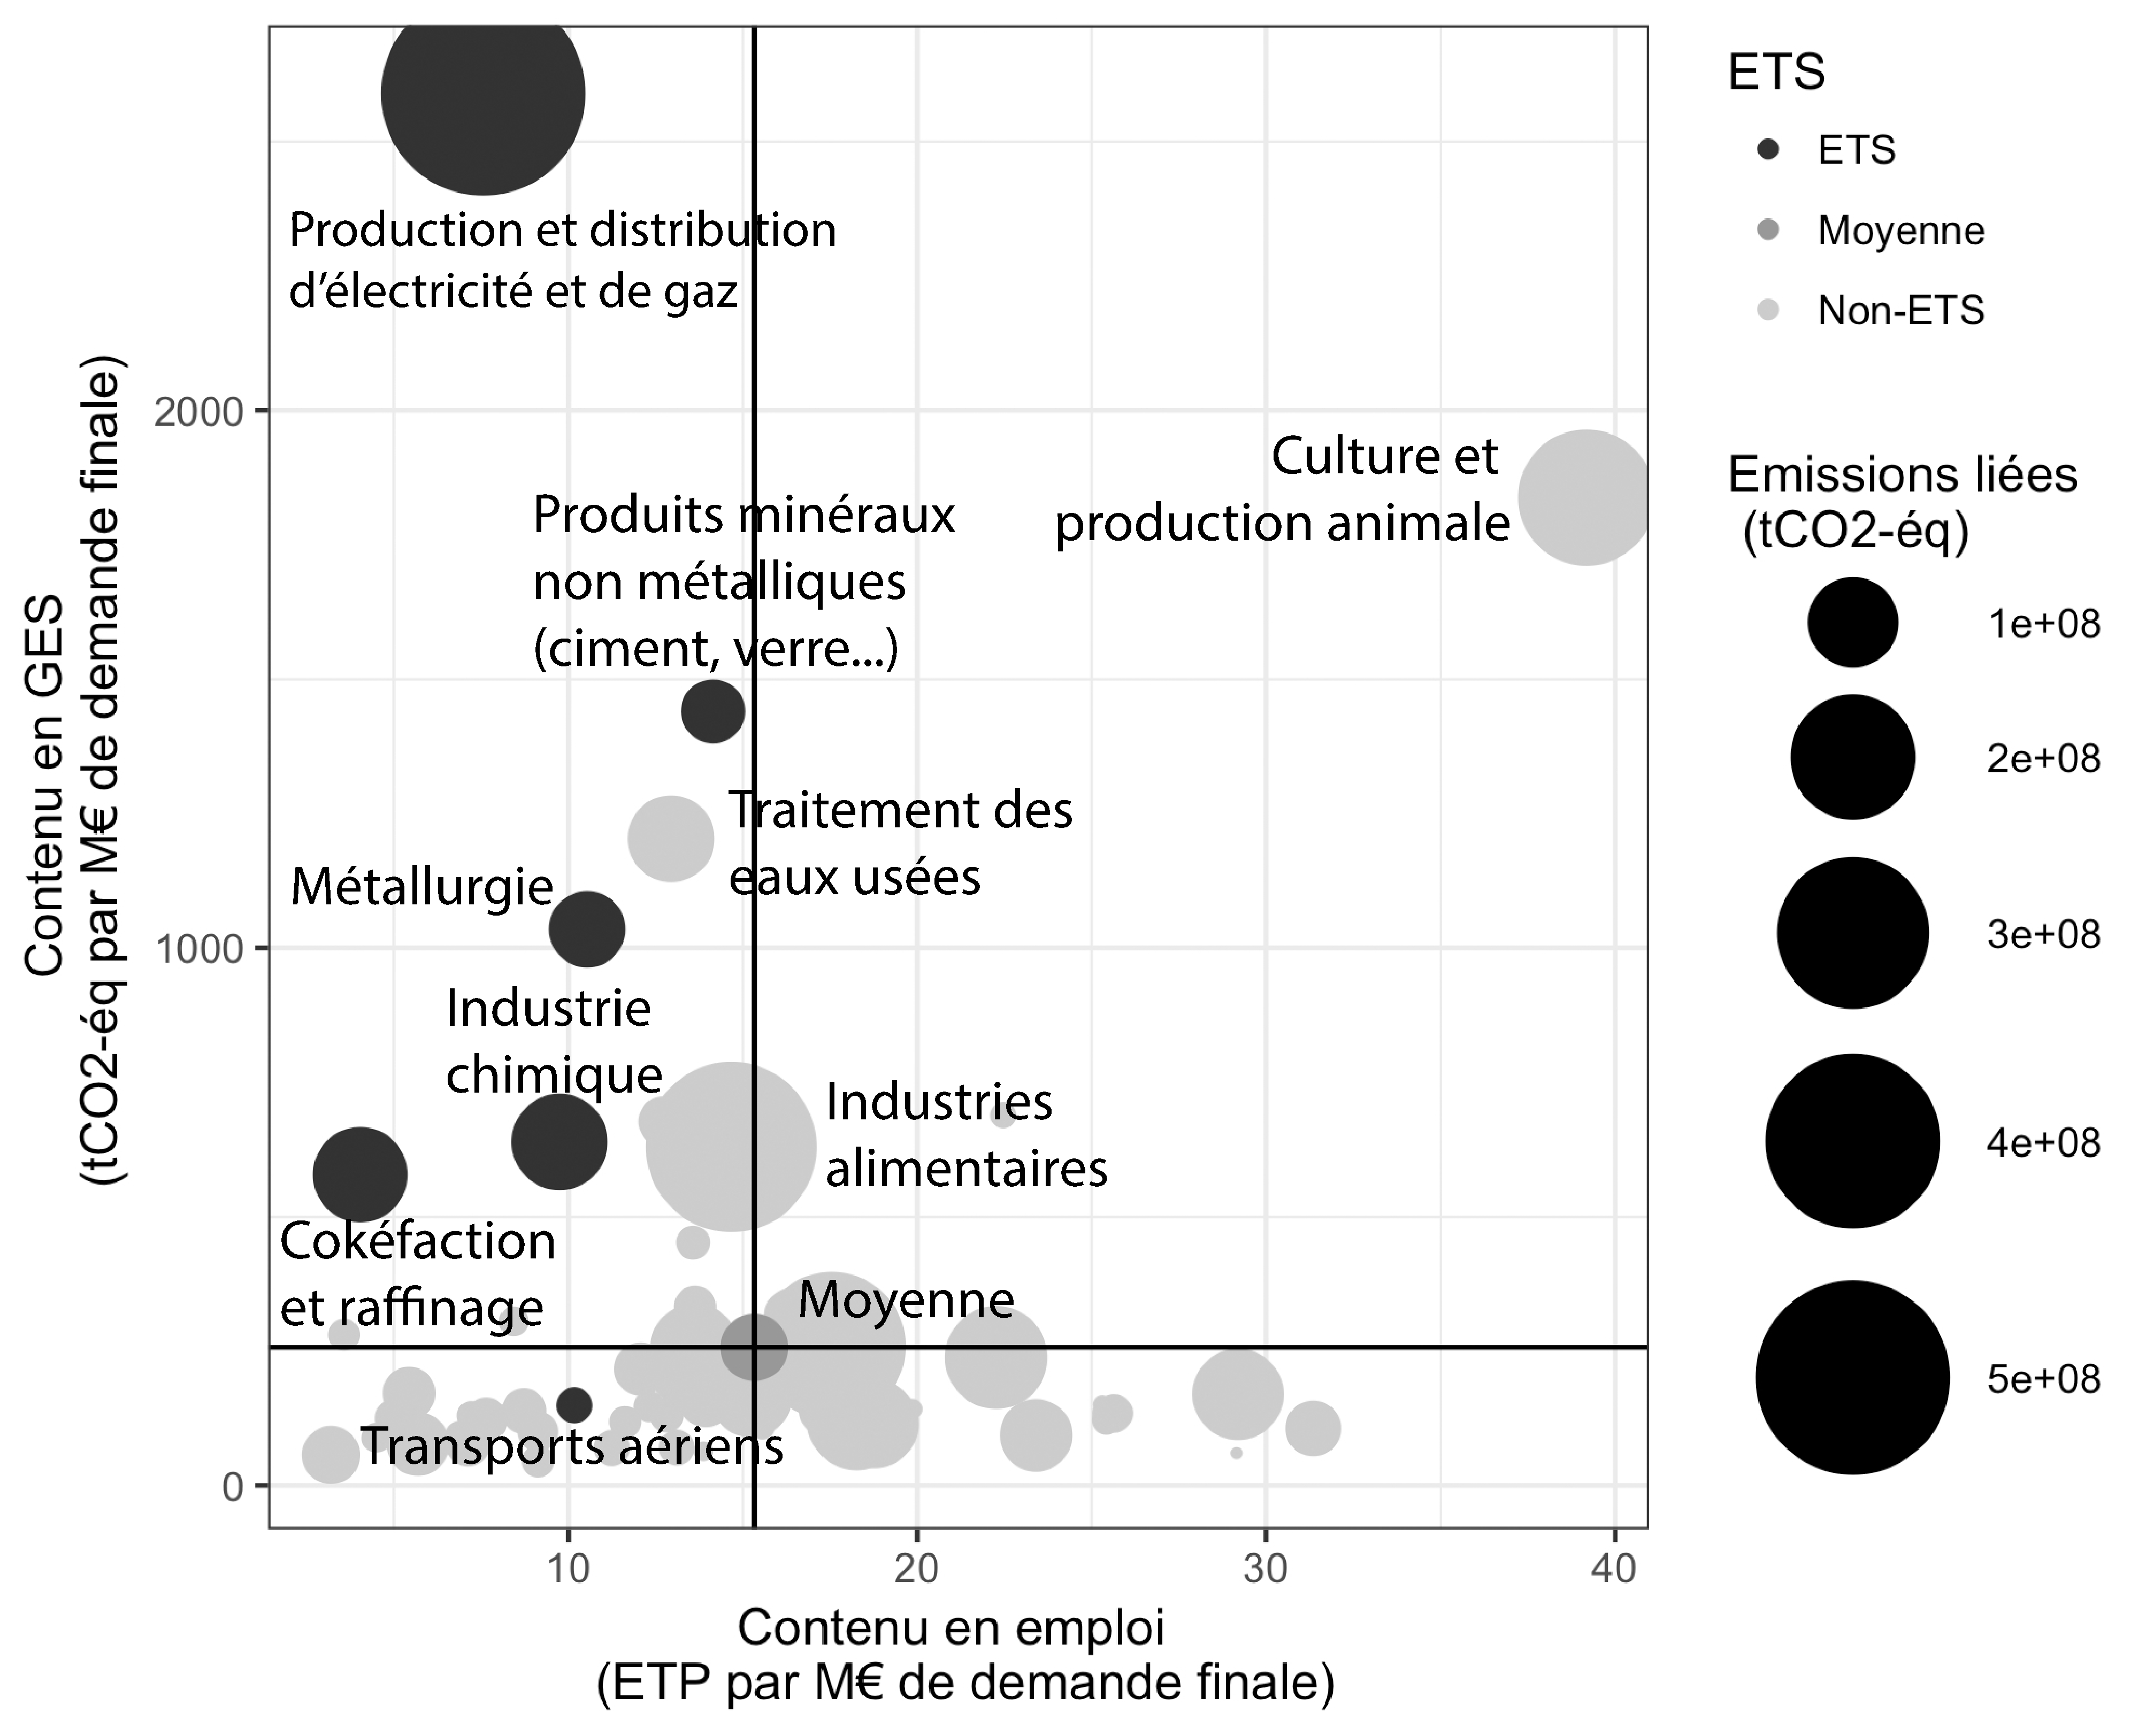
\includegraphics[height=11cm]{figures/GES_et_emplois/GES_emploi_EU.pdf}
	\caption{Contenu en GES et en emploi des 64 branches de l'économie européenne (Union des 27) \\
		Sources : Calcul des auteurs à partir de données Eurostat.}
	\label{fig:ges_emploi_EU}
	\captionsetup{justification=raggedright}
	\caption*{Lecture : ce graphique est identique à la figure \ref{fig:ges_emploi}, mais le périmètre est ici celui des 27 pays membres de l'Union Européenne. On note que la branche "Production et distribution d'électricité et de gaz" est ici beaucoup plus émettrice que pour la France. La présence de nucléaire et d'hydraulique en France explique en grande partie cette différence.}
\end{figure}


\clearpage
\subsection{Graphique incluant les émissions finales des ménages}
\label{app:emissions_menages}

\begin{figure}[!h]
	\centering
	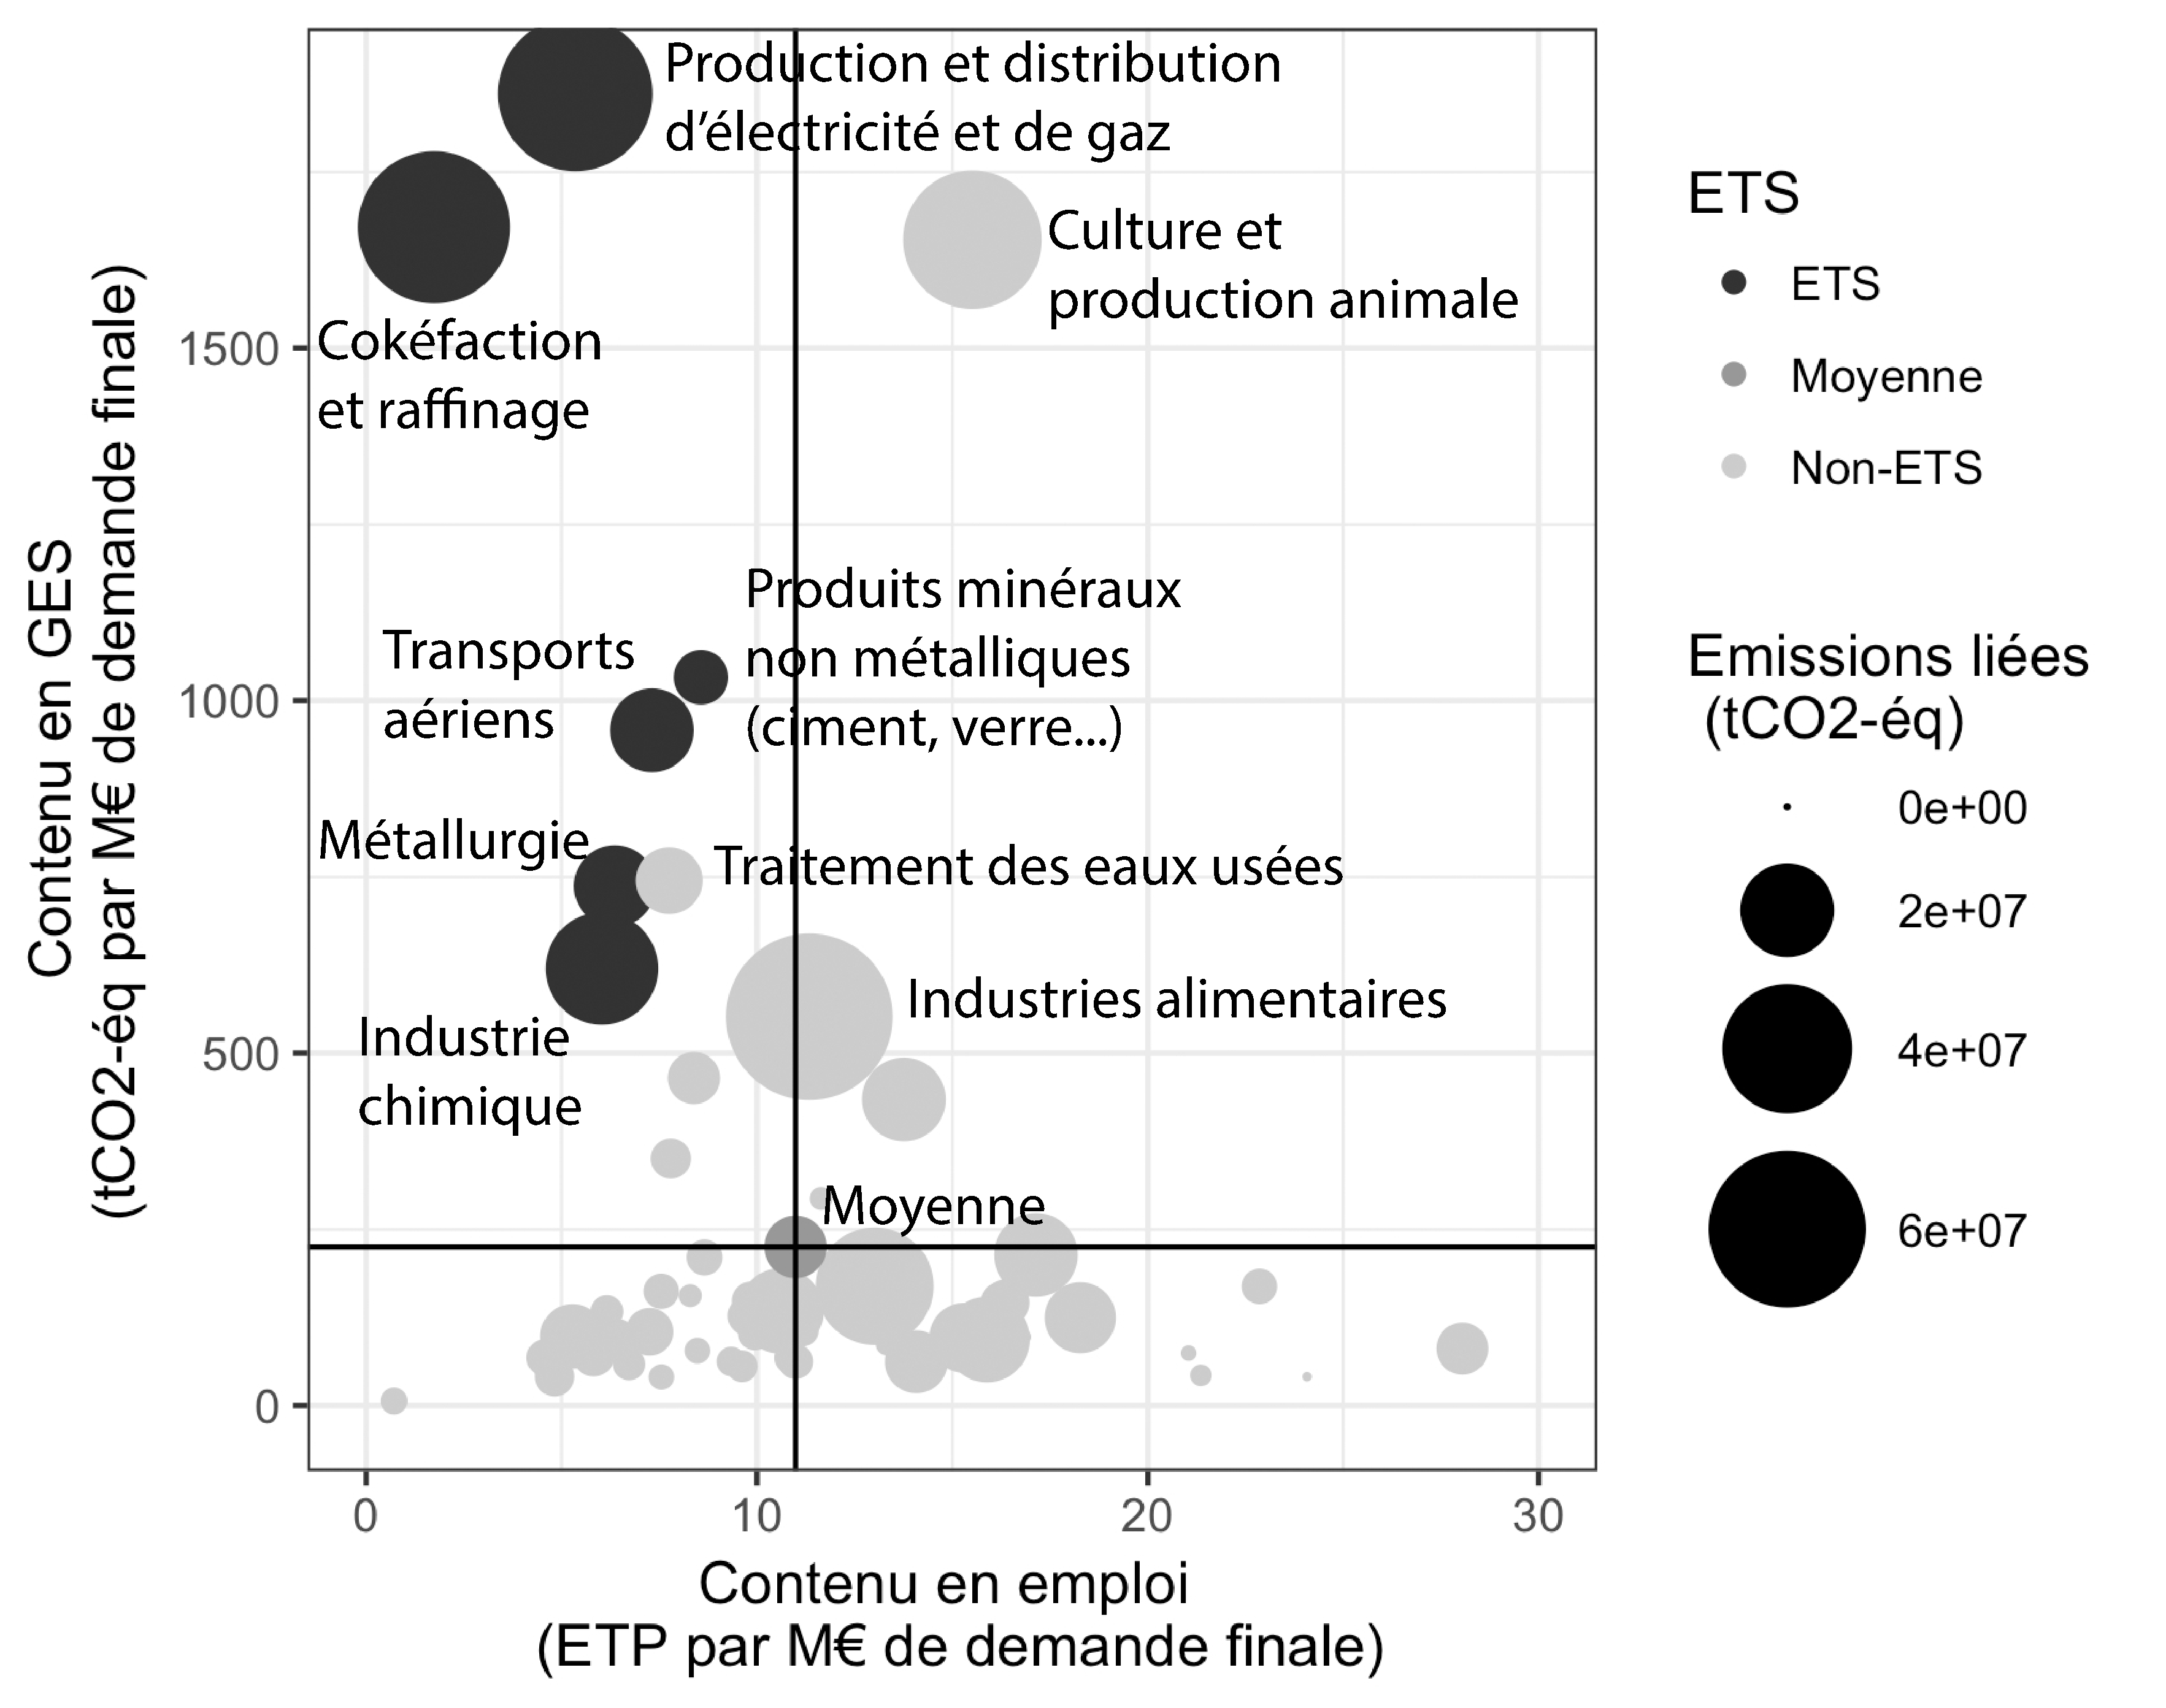
\includegraphics[height=11cm]{figures/GES_et_emplois/GES_menages_emploi.pdf}
	\caption{Contenu en GES et en emploi des 64 branches de l'économie française, en incluant les émissions finales \\
		Sources : Calcul des auteurs à partir de données Eurostat.}
	\label{fig:ges_menages_emploi}
	\captionsetup{justification=raggedright}
	\caption*{Lecture : Cette figure est identique à la figure \ref{fig:ges_emploi}, à la différence près que nous avons incluant les émissions dues aux utilisations finales des ménages. Les émissions des transports ont été affectées en tant qu’émissions directes de la branche « Cokéfaction et raffinage », avant application de la méthode de Leontief. De la même manière, les émissions de chauffage individuel des ménages ont été affectées comme émissions directes de la branche « Electricité, gaz, vapeur ». Les valeurs utilisées sont celles d'Eurostat, base de données env\_ac\_ainah\_r2.}
\end{figure}

\clearpage
\subsection{Contenu en emploi des branches soumises à l'EU ETS}
\label{app:EU_ETS}

\begin{figure}[!h]
	\centering
	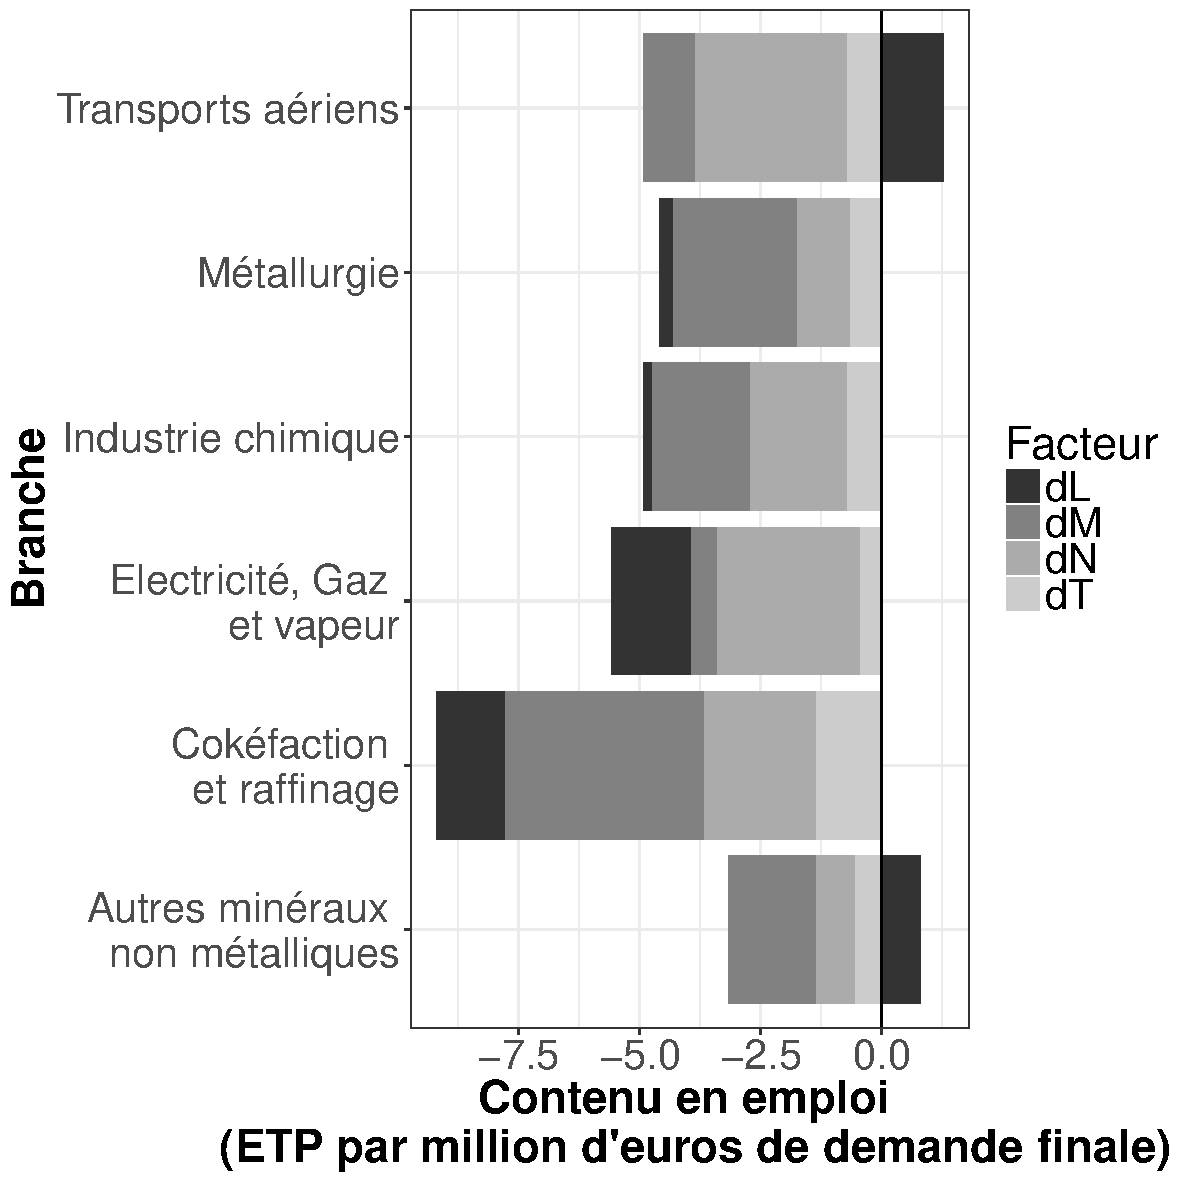
\includegraphics[height=11cm]{figures/GES_et_emplois/EU_ETS.pdf}
	\caption{Décomposition du contenu en emploi dans les branches soumises à l'EU ETS \\
		Sources : Calcul des auteurs à partir de données Eurostat.}
	\label{fig:EU ETS}
	\captionsetup{justification=raggedright}
	\caption*{Lecture : Ce graphique indique la différence entre le contenu en emploi de chaque branche et la moyenne nationale. Nous avons ici agrégé les importations finales et intermédiares : $dM = dMF + dMI$ pour plus de lisibilité. $dL$ indique la part du travail dans la valeur ajoutée, $dN$ le niveau des salaires et $dT$ le niveau de taxes et subventions. On voit que les branches soumises à l'EU ETS ont un contenu en emploi inférieur à la moyenne, principalement du fait d'importations élevées et/ou d'une faible part des salaires dans la valeur ajoutée.}
\end{figure}

